\documentclass[12pt,a4paper]{article}

\usepackage[utf8]{inputenc}
\usepackage{graphicx}
\usepackage{float}

\begin{document}

\title{MI-PAA 2015 1. a 2.ukol}
\author{Tomas Nesrovnal\\nesrotom@fit.cvut.cz}
\date{\today}
\maketitle

\section{Specifikace ulohy}
Problem 0-1 batohu.

\section{Rozbor moznych variant reseni}
Ulohu muzu resit hrubou silou. Ziskam tam presny vysledek, ale vypocet bude
pomaly. Dalsim resenim je pouzit heuristiku, jejiz vyledek nebude nejlepsi mozny
ale vypocet probehne rychle.

\section{Ramcovy popis postupu reseni}
\subsection{Hruba sila}
Zkusim vsechny moznosti a vyberu tu nejlepsi.
\subsection{Heuristika}
Vkladam do bahothu nejlepsi predmety s pomerem cena/vaha, dokud
mi jeste staci kapacita.

\section{Popis kostry algoritmu}
\subsection{Hruba sila}
Vytvorim pole, ktere udava ktery predmet je v batohu. Rekurzivne zkousim
vsechny moznosti (zavolam rekurzi bez prvku, pak prvek pridam a zavolam rekurzi znovu).
Ulozim si nejlepsi reseni.

Druha varianta obsahuje vylepseni: Pokud ve stromu reseni narazim na to, ze se do batohu uz vic nevejde, vetev zariznu.
\subsection{Heuristika}
Seradim si pole s predmety podle pomeru cena/vaha (nebo jine varianty, viz grafy). Cele pole sestupne prochazim a pokud se tam predmet vejde, tak ho tam vlozim.

\section{Namerene vysledky}

\subsection{Spravnost vysledku}
Pomoci skriptu byla overena spravnost vysledku (porovnanim s referencnim resenim).

\subsection{Na cem bylo mereno}
Intel(R) Core(TM) i3-2328M Processor (3M Cache, 2.20 GHz), gcc 4.9.2 (-Ofast), OS GNU/Linux Lubuntu 14.04 64bit

\subsection{Grafy}
Vsechny grafy byly vygenerovany skriptem (error.sh). Cas byl meren pomoci knihovny OpenMPI.
Sript byl spusten pres prikaz \textbf{sudo time nice -n -20 ./error.sh} a trval 180 sekund.

Presna cisla lze nalezt v \textbf{*.plot} souborech.

Chyba heuristiky: Z kazdeho batohu spocitana relativni chyba. V grafu jsou pak secteny relativni chyby pro celou sadu. Celkem 3 heuristiky.

\begin{figure}[H]
	\caption{Doba behu reseni heuristikou (cena/vaha). 5000 opakovani. }
	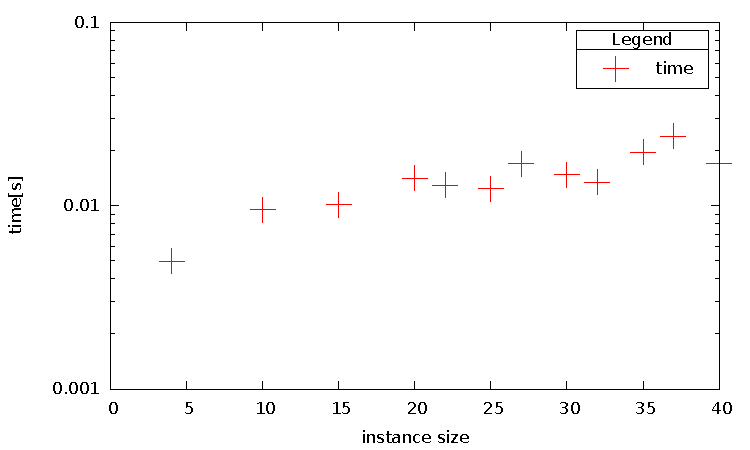
\includegraphics{./time_h1.pdf}
\end{figure}

\begin{figure}[H]
	\caption{Doba behu reseni hrubou silou. 5 opakovani. }
	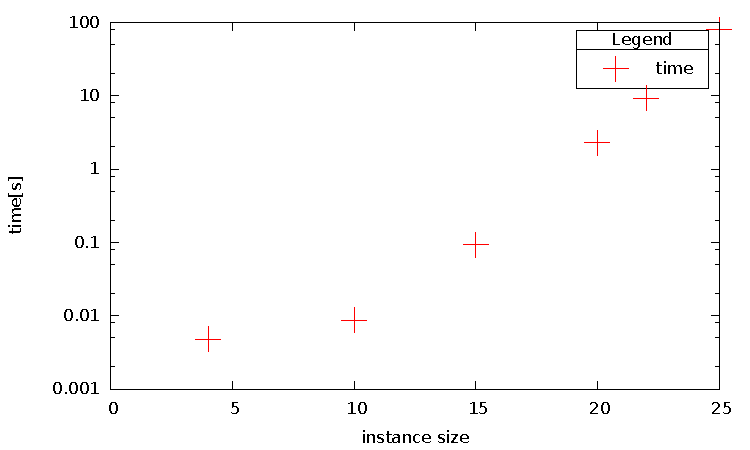
\includegraphics{./time_b0.pdf}
\end{figure}

\begin{figure}[H]
	\caption{Doba behu reseni hrubou silou (s orezavanim). 5 opakovani. }
	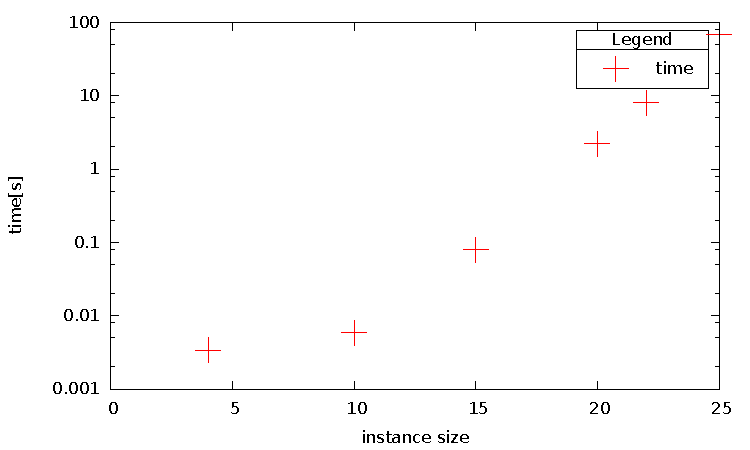
\includegraphics{./time_b1.pdf}
\end{figure}

\begin{figure}[H]
	\caption{heuristika (podle ceho se radilo): pomer cena/vaha}
	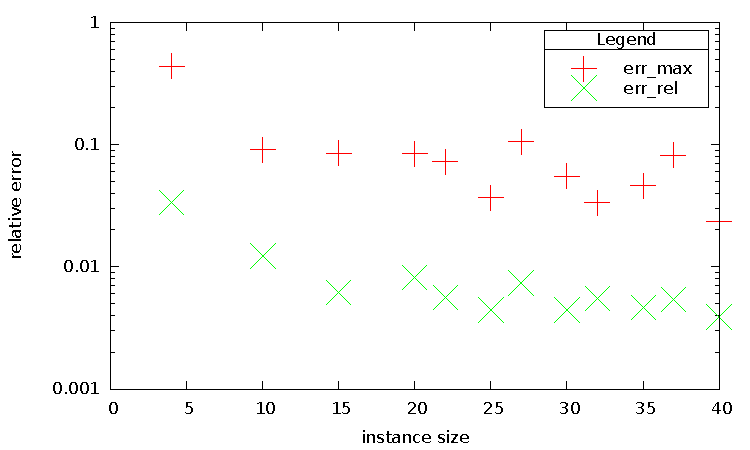
\includegraphics{./err_h1.pdf}
\end{figure}

\begin{figure}[H]
	\caption{heuristika (podle ceho se radilo): cena}
	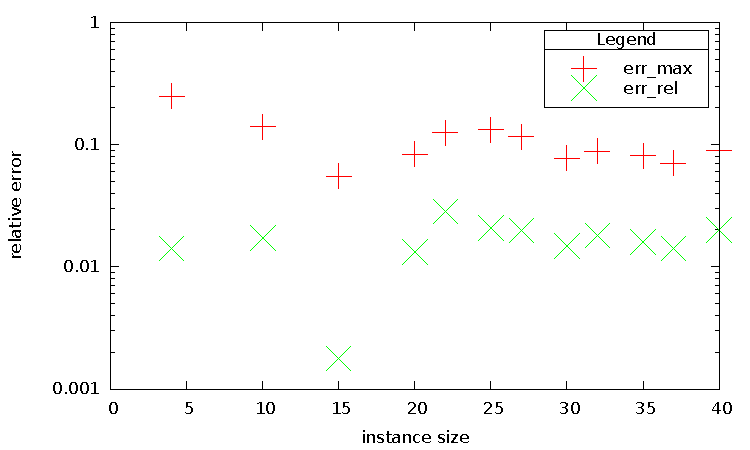
\includegraphics{./err_h2.pdf}
\end{figure}

\begin{figure}[H]
	\caption{heuristika (podle ceho se radilo): vaha}
	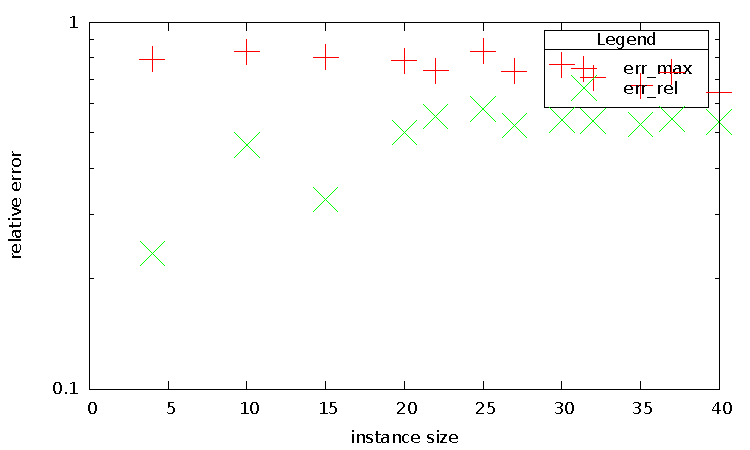
\includegraphics{./err_h3.pdf}
\end{figure}


\section{Zaver 1. uloha}
Vysledky se shoduji s rozborem reseni. Hruba sila je opravdu pomala a byt jednoducha heuristika nevraci zas tak spatne reseni.

Heuristika cena/vaha byla nejlepsi z heuristik.

Orezavani bruteforce melo za nasledek zrychleni o 12 sekund u instance o velikosti 25.

Bruteforce ma slozitost $O(2^n)$, zatimco heuristika jen $O(nlogn)$. Z tohoto duvodu bylo mereni na heuristice opakovano 50000x, zatimco na bruteforce pouze 5x.

Jeste nutno podotknout, ze na takhle malych datech (navic asi nahodne vygenerovanych) muzou byt velke odchylky a anomalie.


\section{2. uloha}

\section{Branch and Bound}
Orezaval jsem ze shora i z dola. Pred tim jsem pole seradil jako v heuristice, aby bylo orezavani efektivnejsi.

\section{Dynamicke programovani}
Implementoval jsem dva zpusoby dymanickeho programovani. Jeden zpusob plnil tabulku od spoda nahoru (dva cykly v sobe).
Druhy resil odshora dolu (rekurze). Obe reseni vracely spravne vysledky, ale prvni zpusob byl mnohem rychlejsi.

Obe tyto reseni meli dekompozici podle vahy.

\section{FPTAS}
FPTAS je podobny heuristice. Nejdriv ale spocitam maximalni chybu a podle toho a podle nastavene mozne chyby epsilon preskaluji vstupni data. Pro chybu eps=0 byly tedy vysledky spravne, stejne jako u dynamickeho programovani.


\section{Zaver 2. uloha}
BB vyrazne pomohla, ale je hodne citliva na vstupni data.

Dynamicke programovani je lepsi (dle namerencyh udaju) provadet odspoda a je lepsi se vyhnout rekurzi.

FPTAS pocita s chybou, ale pri dobre zvolenem eps mame malou chybu a rychle reseni.

\section{Grafy}

Nasleduje kompletni vycet grafu, kde time ukazuje  rychlost vypoctu (pro pomale alrogritmy nebyly pouzite velke instance). "err" ukazuje chybu. f znamena algoritmus FPTAS a cislo za nim je nastavene eps v procentech. d je dynamicke programovani, 1 je shora dolu, 2, z dola nahoru. b je bruteforce. b0 je neoptimalizovane, b1 s BB. h je heuristika jeste z prvni ulohy.

\begin{figure}[H]
\caption{time\_f0.pdf }
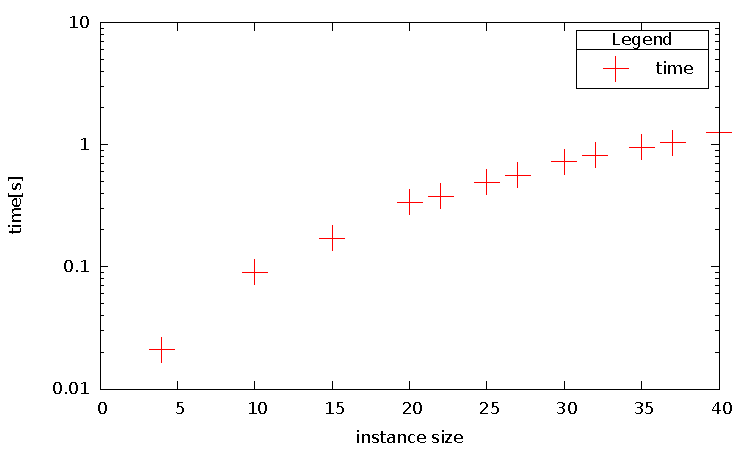
\includegraphics{./time_f0.pdf}
\end{figure}

\begin{figure}[H]
\caption{time\_f25.pdf }
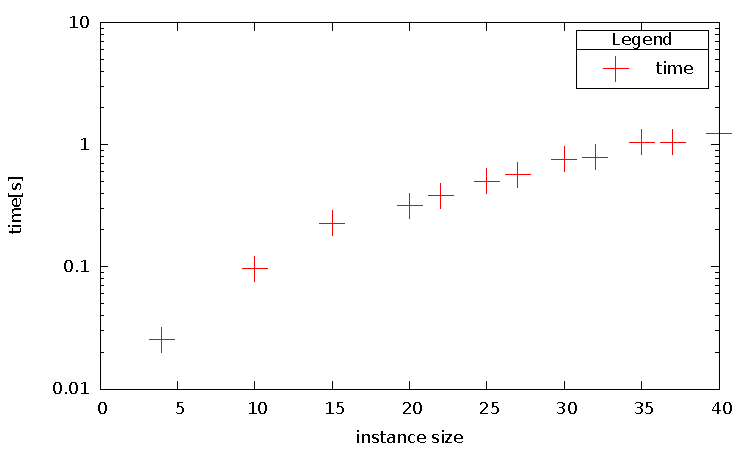
\includegraphics{./time_f25.pdf}
\end{figure}

\begin{figure}[H]
\caption{time\_f50.pdf }
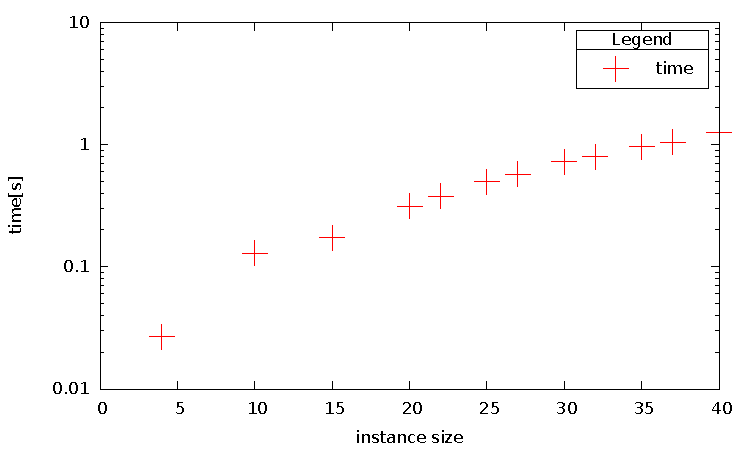
\includegraphics{./time_f50.pdf}
\end{figure}

\begin{figure}[H]
\caption{time\_f75.pdf }
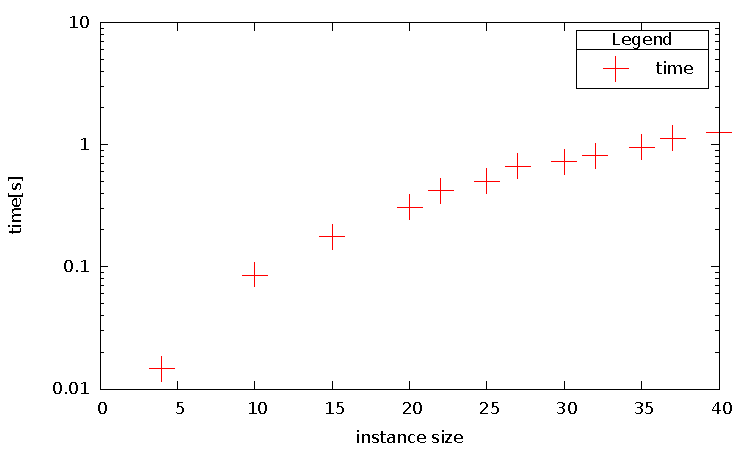
\includegraphics{./time_f75.pdf}
\end{figure}

\begin{figure}[H]
\caption{time\_f100.pdf }
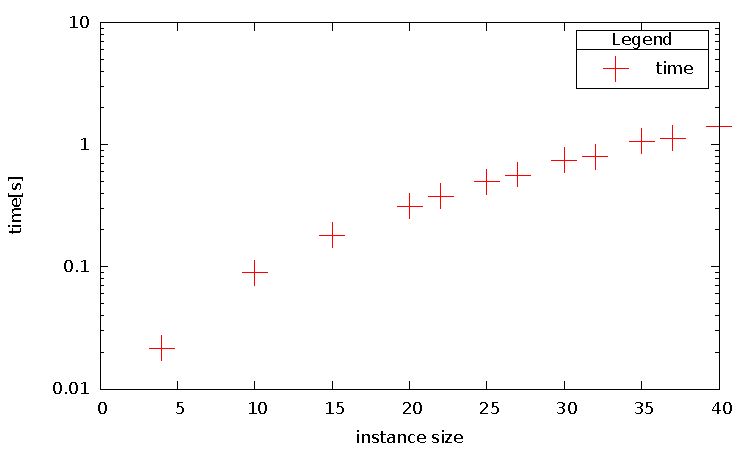
\includegraphics{./time_f100.pdf}
\end{figure}

\begin{figure}[H]
\caption{time\_d1.pdf }
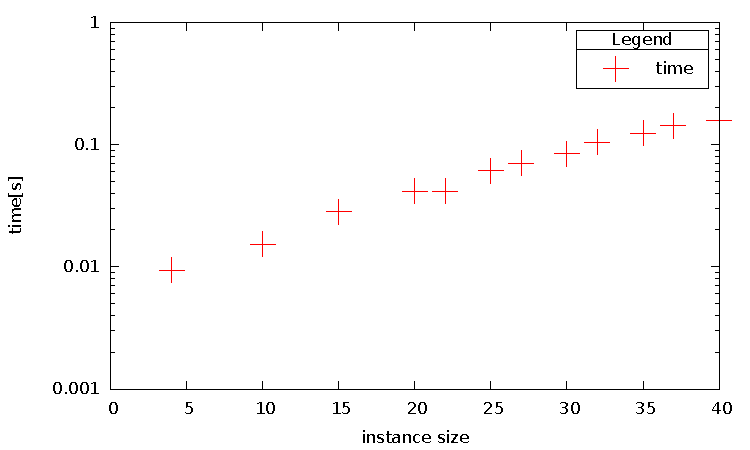
\includegraphics{./time_d1.pdf}
\end{figure}

\begin{figure}[H]
\caption{time\_d2.pdf }
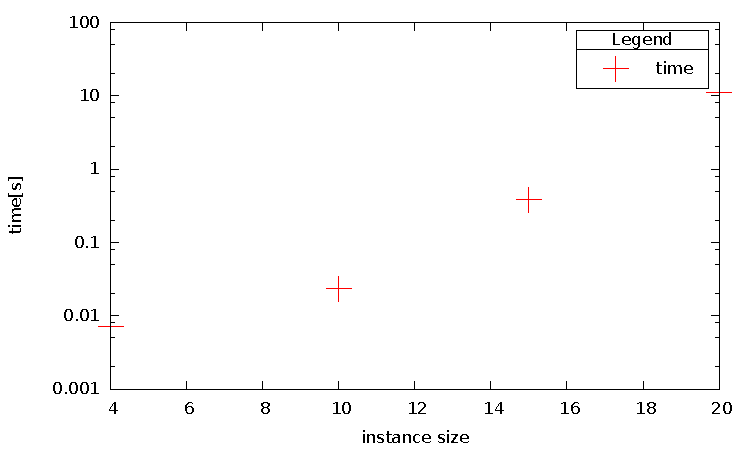
\includegraphics{./time_d2.pdf}
\end{figure}

\begin{figure}[H]
\caption{time\_b0.pdf }
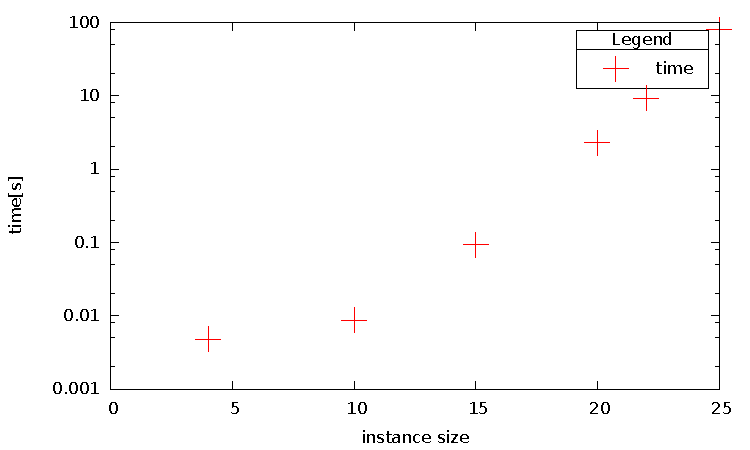
\includegraphics{./time_b0.pdf}
\end{figure}

\begin{figure}[H]
\caption{time\_b1.pdf }
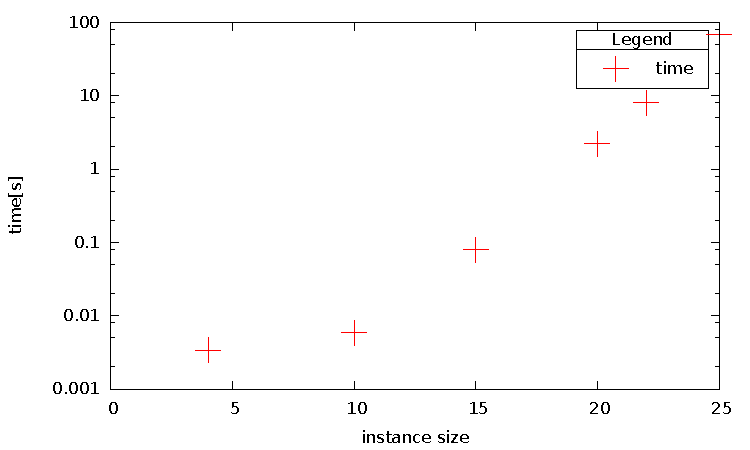
\includegraphics{./time_b1.pdf}
\end{figure}

\begin{figure}[H]
\caption{time\_h1.pdf }
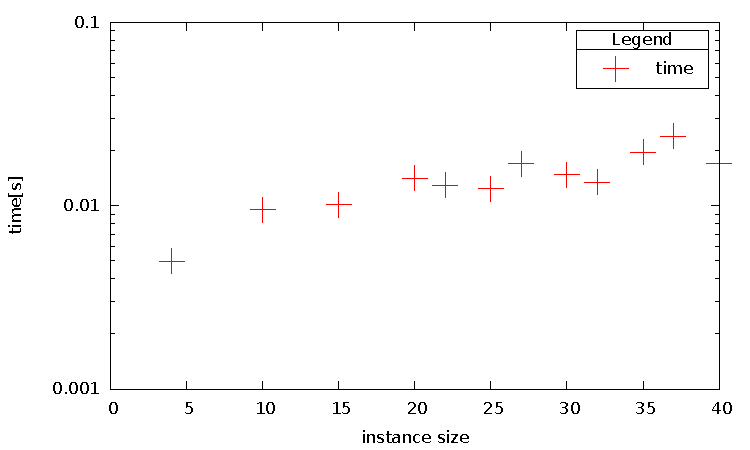
\includegraphics{./time_h1.pdf}
\end{figure}

\begin{figure}[H]
\caption{time\_h2.pdf }
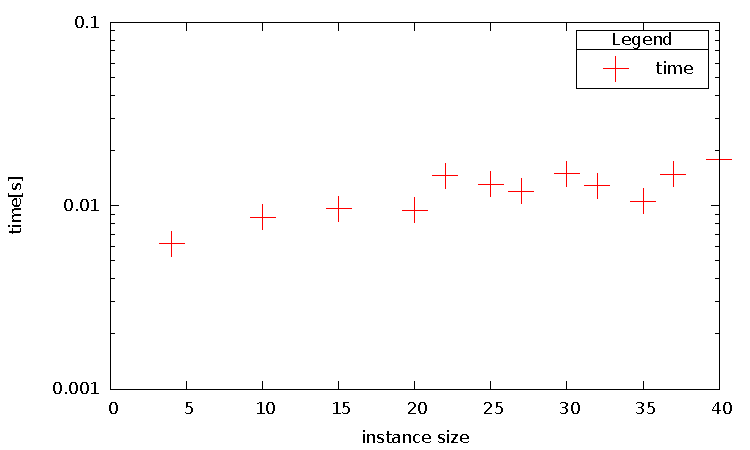
\includegraphics{./time_h2.pdf}
\end{figure}

\begin{figure}[H]
\caption{time\_h3.pdf }
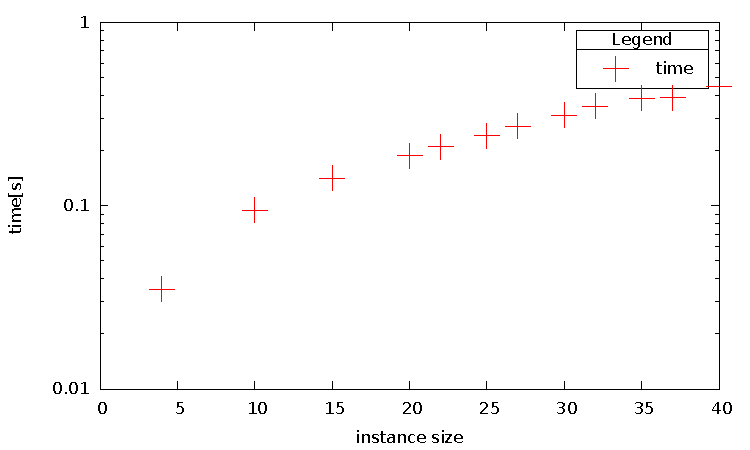
\includegraphics{./time_h3.pdf}
\end{figure}

\begin{figure}[H]
\caption{err\_f25.pdf }
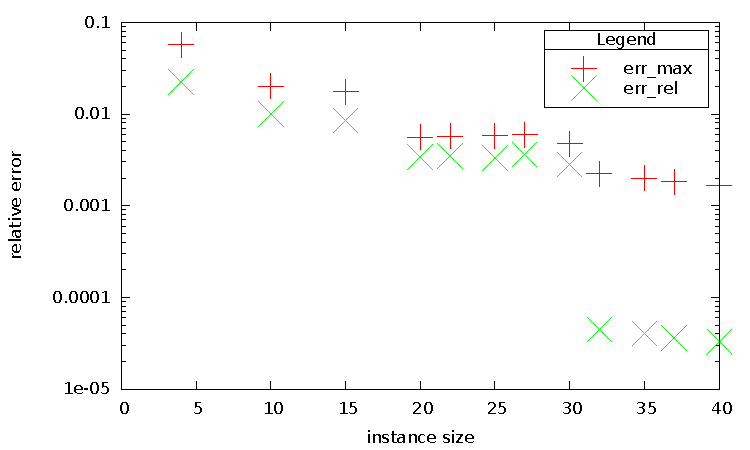
\includegraphics{./err_f25.pdf}
\end{figure}

\begin{figure}[H]
\caption{err\_f50.pdf }
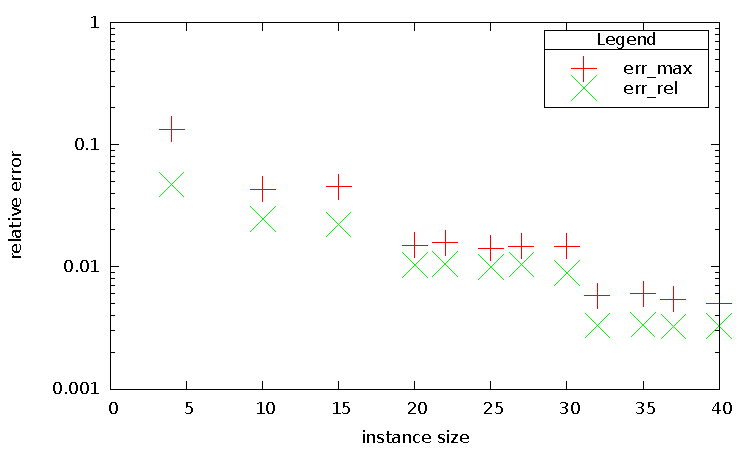
\includegraphics{./err_f50.pdf}
\end{figure}

\begin{figure}[H]
\caption{err\_f75.pdf }
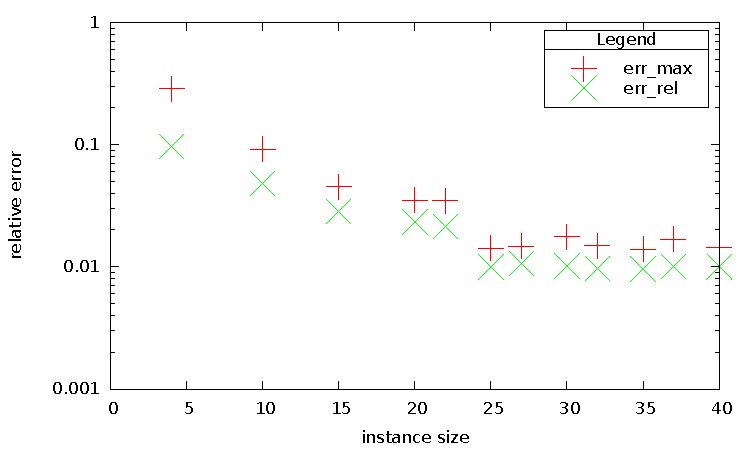
\includegraphics{./err_f75.pdf}
\end{figure}

\begin{figure}[H]
\caption{err\_f100.pdf }
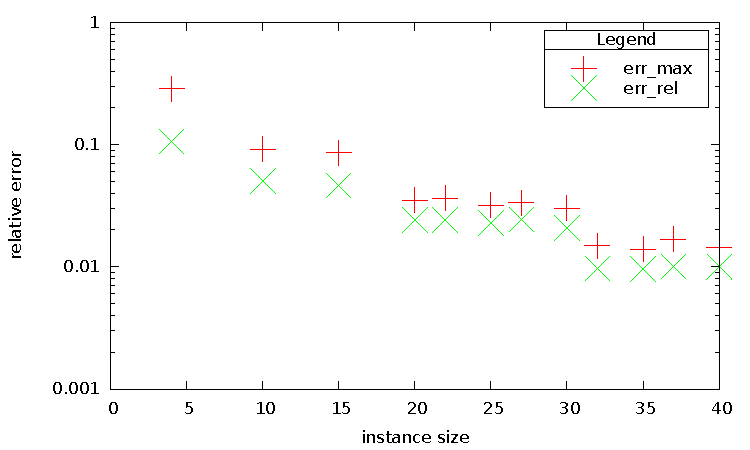
\includegraphics{./err_f100.pdf}
\end{figure}

\begin{figure}[H]
\caption{err\_h1.pdf }
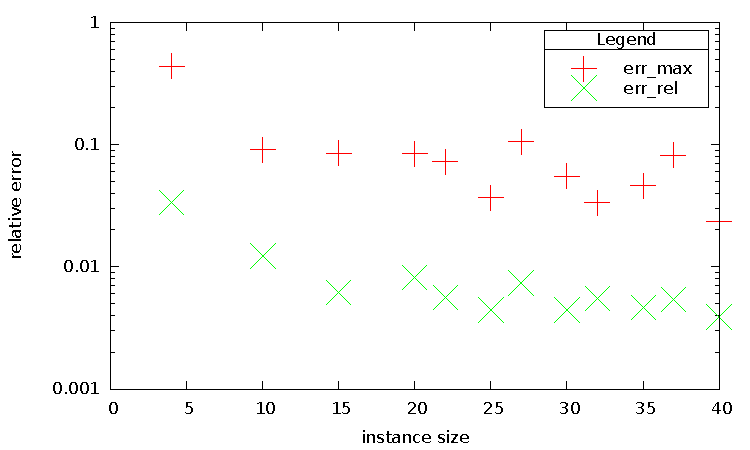
\includegraphics{./err_h1.pdf}
\end{figure}

\begin{figure}[H]
\caption{err\_h2.pdf }
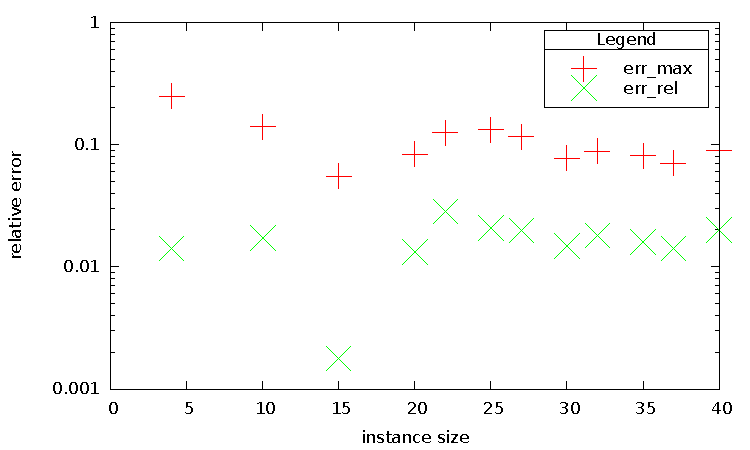
\includegraphics{./err_h2.pdf}
\end{figure}

\begin{figure}[H]
\caption{err\_h3.pdf }
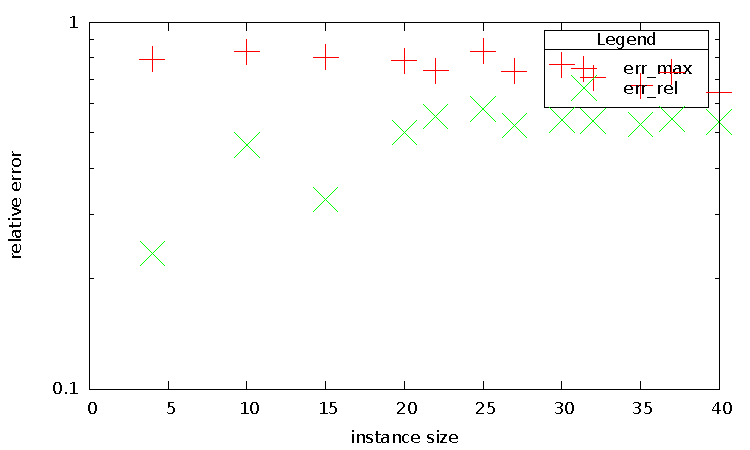
\includegraphics{./err_h3.pdf}
\end{figure}


%%%%%%%%%%%%%%%%%%%%%%%%%%%%%%%%%%%%%%%%%%%%%%%%%%%%%%%%
\end{document}
